\chapter{Vergelijkingscriteria}
\label{chap:vergelijkingscriteria}

Dit hoofdstuk bekijkt hoe de mobiele HTML5 raamwerken actief zullen worden vergeleken.
Hoofdzakelijk zal dit gebeuren aan de hand van een \term{proof of concept}~(POC).
Deze wordt geïntroduceerd in sectie \ref{sec:vergelijking-poc} en zal hoofdzakelijk de gekozen vergelijkingscriteria in sectie \ref{sec:vergelijking-criteria} drijven.
De criteria die worden voorgesteld, zullen voortaan actieve criteria worden genoemd.


\section{POC}
\label{sec:vergelijking-poc}
In samenspraak met Capgemini werd gekozen om een \term{proof of concept}~(POC) op te stellen.
%TODO hier refereren en reflecteren over POC in literatuur (tim)
Dit is een idee waarbij de uitvoerbaarheid in de verschillende raamwerken kan worden nagegaan.
Verschillende vergaderingen werden georganiseerd om tot een idee te komen dat vooral in de bedrijfswereld van toepassing is.
Het uiteindelijke idee is een applicatie die het mogelijk maakt voor werknemers om hun onkosten via hun mobiel apparaat door te sturen.

Het idee werd uitgewerkt door Capgemini en geleverd aan de auteurs als \term{mockup}.
Dit is een voorstelling van de applicatie als een reeks schermen zoals deze er zullen uitzien op een apparaat. 
Een voorbeeld van zo een scherm is te vinden op figuur~\ref{fig:poc}. 
Naast de schermen staan de functionele vereisten die op het scherm van toepassing zijn.
De bedoeling is dat deze POC wordt uitgewerkt zowel voor smartphone als tablet, zowel voor Android als iOS, zowel voor staande als liggende apparaten en zowel voor online als offline gebruik.

\begin{figure}
  \centering
  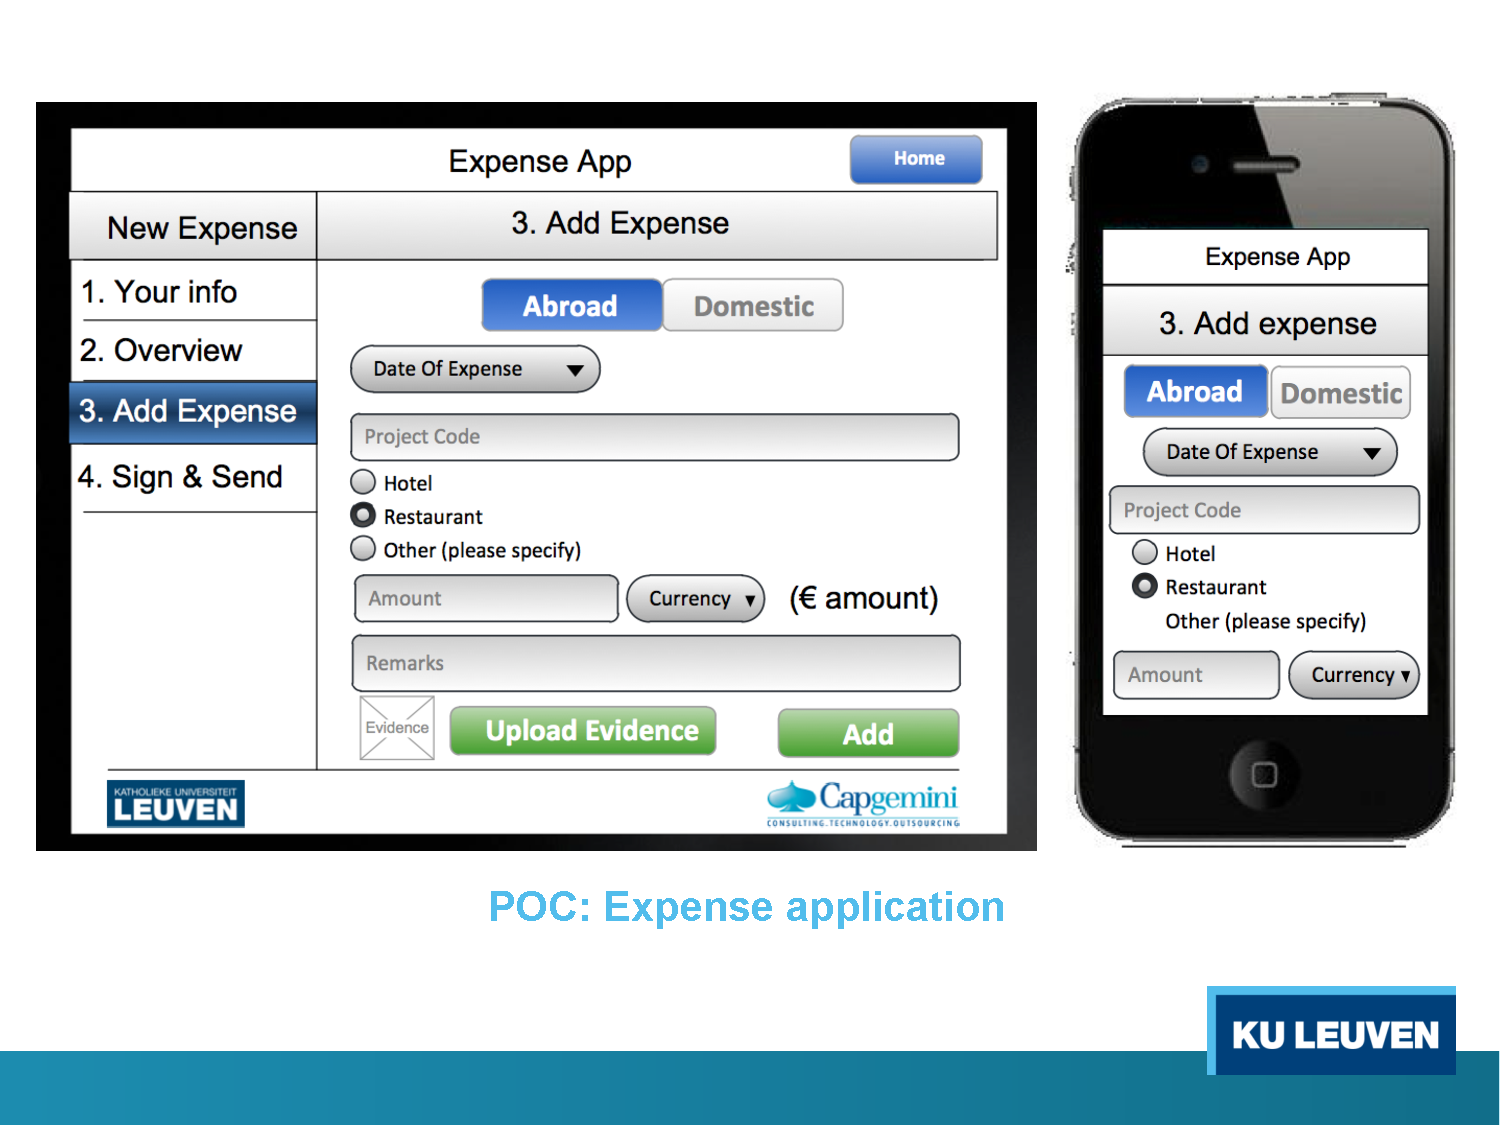
\includegraphics[trim=0cm 4.6cm 0cm 1.55cm,clip=true,width=\textwidth]{figuren/poc.pdf}
  \caption{POC bij het toevoegen van een nieuwe onkost met aan de linkerkant de weergave op een tablet en aan de rechterkant deze op een smartphone.}
  \label{fig:poc}
\end{figure}

\subsection{Aspecten}
\label{sec:vergelijking-poc-detail}

Een werknemer meldt zich eerst aan op de applicatie en kan daarna ofwel een nieuw onkostenformulier aanmaken of zijn doorgestuurde onkostenformulieren bekijken.
De term onkostenformulier is een groepering van meerdere onkosten met bijhorende bewijsstukken en de handtekening van de werknemer. 
Het aanmaken van een nieuw onkostenformulier verloopt in vier stappen.
Indien de werknemer al eerder begonnen was met het aanmaken van een formulier, zal hij worden gevraagd of hij verder wil gaan met dat formulier of met een nieuw formulier wil starten.

\begin{enumerate}
\item De eerste stap is het bekijken en/of aanpassen van de persoonlijke informatie van de werknemer.
Bij het aanpassen van deze gegevens, zullen deze worden gevalideerd.
Indien deze validatie faalt, krijg de werknemer een dialoogvenster te zien met de reden tot falen.
Ook worden de foute velden rood gemarkeerd.

\item In de tweede stap kan de werknemer zijn toegevoegde onkosten aan het formulier bekijken.
In het begin is deze lijst leeg, tenzij hij eerder een formulier aan het invullen was (zie infra).
Indien deze lijst onkosten bevat, is het mogelijk om hierop te klikken en deze te bekijken.
Aanpassen is niet mogelijk.

\item In stap drie kan een nieuwe onkost worden toegevoegd.
Dit kan ofwel een binnenlandse ofwel buitenlandse onkost zijn.
Voor beide dient een datum en projectcode te worden opgegeven.
De eerstgenoemde is een \term{datepicker} die teruggaat tot twee maanden in de tijd.
De laatstgenoemde bevat automatische aanvulling, maar de werknemer is niet verplicht om een projectcode uit de aanvulling te selecteren.
Daarnaast dient het type en bedrag van de onkost, alsook een bewijsstuk te worden opgegeven.
Bij een buitenlandse onkost moet de munteenheid worden opgegeven, waarna de applicatie deze automatisch omvormt naar euro.
Het scherm voor het toevoegen van een buitenlandse onkost wordt getoond op figuur \ref{fig:poc}. 
Net zoals bij stap één geldt ook hier validatie op de formuliervelden.

\item In deze laatste stap dient een handtekening te worden geplaatst waarna het formulier kan worden doorgestuurd.
Indien de gebruiker offline werkt, zal deze worden opgeslagen op het toestel.
De werknemer kan het formulier opnieuw doorsturen zodra hij terug online is.

\end{enumerate}

Bij het bekijken van de doorgestuurde formulieren is het mogelijk om per formulier de bijhorende PDF te downloaden. 
Deze bevat een overzicht van de onkosten met bijhorende bewijsstukken, alsook de handtekening van de werknemer.

\section{Criteria}
\label{sec:vergelijking-criteria}

In deze sectie zullen de actieve criteria toegelicht worden die zullen worden toegepast om de raamwerken te vergelijken.
In sectie \ref{sec:vergelijken-raamwerken} werden reeds technieken besproken die in de literatuur worden toegepast.
Elementen van deze technieken zullen terugkomen in de voorgestelde methode om de raamwerken te evalueren.
%TODO in elke sectie van een criteria een referentie naar literatuur (zie drive document) + reflecteren met ISO (sander)
Sectie \ref{sec:raamwerken-tabel} bevatte de passieve vergelijkingscriteria die raamwerken vergeleken met informatie over het raamwerk zelf.

Vijf criteria zullen worden gebruikt: populariteit (\ref{sec:vergelijking-populariteit}), productiviteit (\ref{sec:vergelijking-productiviteit}), gebruik (\ref{sec:vergelijking-gebruik}), ondersteuning (\ref{sec:vergelijking-ondersteuning}) en performantie (\ref{sec:vergelijking-performantie}). 
%TODO refereren naar puntensysteem literatuur(tim)
Elk raamwerk krijgt voor elk criterium een score afgeleid uit een formule. 
Deze scores zullen in een spinnenweb worden ondergebracht (zie sectie \ref{sec:vergelijking-spinnenweb}).
Zoals hierboven vermeld zal een POC gebruikt worden bij de vergelijking.
De implementatie van deze POC zal het gebruiks- en ondersteuningscriterium drijven.  
Dit komt omdat Capgemini de POC zo heeft opgesteld dat het de verschillende functionaliteiten bevat die van een normale applicatie verwacht worden.

%TODO populariteit in visionmobile gebruiken bij onze criteria (sander)
\subsection{Populariteit}
\label{sec:vergelijking-populariteit}
%TODO referenties zijn naar blogposts (sander)
De populariteit van een raamwerk is een belangrijke factor want het bepaalt de gemeenschap en levendigheid van het raamwerk.
Het is in cijfers uit te drukken door gebruik te maken van sociale netwerken. 
Een tabel zal voorzien worden met in de rijen het aantal volgers op Twitter, sterren en \term{forkers} van \gh{},  vragen op \so{} en aantal vind-ik-leuks van \fb{}.
%Community: Saffari (codefession)
%SO en google trends: Ayuso (monocaffe)
%\cite{Hales2012}: twitter en github forkers and watchers
%facebook zelf

GitHub kan worden gezien als een sociaal netwerk voor programmeurs~\cite{Catone2008} en bepaalt dus de actieve gemeenschap rond het raamwerk.
Raamwerken die niet op GitHub te vinden zijn krijgen nul voor zowel het aantal sterren en \term{forkers}.
Een alternatief hield de interpolatie van de GitHub data van de overige raamwerken in.
Omdat deze aanpak het raamwerk onterecht zou bevoordelen, is hier niet voor gekozen.

De som van Twitter volgers ($T_r$), \gh{} sterren ($S_r$), \gh{} \term{forkers} ($F_r$), \so{} vragen ($SO_r$) en \fb{} vind-ik-leuks ($FB_r$) vormt de score voor het populariteitscriterium:
\begin{equation}
  \text{Populariteit}_r=T_r+S_r+F_r+SO_r+FB_r
  \label{eq:populariteit}
\end{equation}
voor een raamwerk $r$.

Omdat deze gegevens zeer dynamisch zijn, zullen verschillende metingen in de tijd de evolutie van de data weergeven.
Ook zullen de uitkomsten van dit criterium worden vergeleken met data geleverd door Google Trends~\cite{Google2012a}.
Deze webapplicatie toont de evolutie van zoektermen op Google op een schaal van 100, waarbij 100 overeenkomt met de grootste zoekinteresse.
Voor elk raamwerk zal het aantal zoekopdrachten op Google in functie van de tijd worden uitgezet.

Er bestaat geen exacte formule om populariteit uit te drukken.
De formule die werd gekozen om de score voor dit criterium te quoteren is onderheven aan subjectiviteit.
Twee opmerkingen moeten hierbij worden gemaakt.
Enerzijds zijn de auteurs zich ervan bewust dat de doorsnede tussen sociale netwerken niet leeg is.
Zo kan éénzelfde persoon zowel een volger op Twitter zijn als een vind-ik-leuk op \fb{} plaatsen.
Verschillende individuen zullen dus dubbel geteld worden in de totale score voor populariteit van het raamwerk.
De score zal dus slechts een indicatie geven over de populariteit,  het is geen exacte weergave.
Ten tweede zijn de auteurs er zicht van bewust dat de inclusie van \so{} op twee manieren kan worden bekeken.
Enerzijds kunnen veel vragen duiden op veel onduidelijkheden over het raamwerk.
Anderzijds kan dit een maat zijn voor de populariteit van dit onderwerp.
De auteurs zijn van mening dat de tweede zienswijze correcter is dan de eerste en het dus valide is \so{} in de formule op te nemen.

%%%%%%%%%%%%%%%%%%%%%%%%%%%%%%%%%%%%%%%%%%%%%%%%%%%%%%%%%%%%%%%%%%
%%%%%%%%%%%%%%%%%%%%%%%%%%%%%%%%%%%%%%%%%%%%%%%%%%%%%%%%%%%%%%%%%%

\subsection{Productiviteit}
\label{sec:vergelijking-productiviteit}
%TODO geen eenduidige manier + perceptie
De productiviteit moet berekend hoe lang het duurt om met het raamwerk vertrouwd te raken en iets nuttig te kunnen bouwen.
Dit is belangrijk want bedrijven willen zo min mogelijk tijd verliezen om met nieuwe technolgieën aan de slag te kunnen.
In de ISO 25010-standaard is de categorie van bruikbaarheid vergelijkbaar met dit criterium

De auteurs zullen elk de POC in twee verschillende raamwerken maken en daarnaast ook een extra loginapplicatie in twee andere raamwerken.
De ene auteur maakt de POC in \jqm{} en \lungo{} en de loginapplicatie in \st{} en \kendo{}.
De andere zal dan de POC in \st{} en \kendo{} maken en de loginapplicatie in \jqm{} en \lungo{}.
De tijd die nodig is om de volledige POC te implementeren is een indicatie voor de productiviteit. 
Er wordt verondersteld dat de auteurs over een gemeenschappelijke technische achtergrond beschikken.
Toch kunnen beide onderling verschillen in efficiëntie,  waardoor de productiviteit verschilt.
Dit probleem is inherent aan dit criterium.
Toch is het belangijk om een schatting op deze manier te kunnen maken.

% Omdat de POC twee keer moet worden geïmplementeerd, wordt verwacht dat de tweede implementatie sneller zal verlopen.
% Dit probleem is onafwendbaar en zal bij de evaluatie van de data aangehaald worden.
% De uren voor de implementatie van de loginapplicatie zal de score correcter maken.
% 
% De som van de uren voor het implementeren van de POC ($t_{r,POC}$) en de loginapplicatie ($t_{r,login}$) vormt de score voor de productiviteit:
% \begin{equation}
%   \text{Productiviteit}_r = {t_{r,POC} + t_{r,login}}
%   \label{eq:productiviteit}
% \end{equation}
% voor een raamwerk $r$.

Er zijn echter vijf redenen waarom de implementaties van de POC geen goede indicatie zijn voor de productivteit.
Deze werden door de auteurs ervaren wanneer de implementatie in het tweede raamwerk werd uitgevoerd:
\begin{enumerate}
\item Betere ervaring met de POC versnelt bij de tweede implementatie het overzicht van vereisten die moeten worden geïmplementeerd. 
\item Een verbeterde ervaring met HTML5-raamwerken had een positieve invloed op de verdere implementaties.
Dit weerspiegelde zich vooral tussen \jqm{} en \lungo{}.
Hoewel ze beide op een verschillende \js{}-bibliotheek steunen - respectievelijk jQuery en QuoJS - zijn de gelijkenissen tussen deze twee raamwerken groot.
Ook leggen ze beide geen architectuur op.
\item Er kon code,  zoals van de implementatie in \jqm{},  overgenomen worden bij de implementatie van de POC met \lungo{} en \kendo{}.
\item Er kwamen bij de eerste implementatie problemen met de \term{backend} naar boven.
Deze waren bij de tweede implementatie reeds opgelost.
Door het onnauwkeurig opmeten van de tijd kan er geen schatting worden gemaakt van de tijd die aan de problemen van de \term{backend} werden besteed.
\item Niet de volledige POC kon met \lungo{} en \st{} worden ontwikkeld.
\end{enumerate}

De implementatie van de loginapplicatie is een alternatieve test van de productiviteit.
Deze applicatie bevat GI-elementen, validaties,  \term{backend} integratie en een lijst.
De implementatie van de loginapplicatie kan dus als voldoende steekproef beschouwd worden om ervaring met een raamwerk te testen.
Na het aanmelden met deze applicatie zal de gebruiker een lijst van $850$ elementen te zien krijgen.
Deze lijst is bedoeld als stresstest om de performantie te testen (zie sectie \ref{sec:vergelijking-performantie}).
De elementen in de lijst zullen voorzien worden van een afbeelding en tekst.
De lijst kan als een potentiële muziekapplicatie gezien worden waarbij de afbeelding en tekst naar liedjes verwijzen.
Het aantal elementen in de lijst - $850$ - is een schatting van het maximum aantal liedjes dat ooit is opgenomen~\cite{Zimmy2011}.
Het kan dus als bovengrens voor dit soort applicaties worden beschouwd.
De implementatie van deze applicatie zal een indicatie geven hoe snel,  zonder al te veel voorkennis van het raamwerk,  één eenvoudige applicatie opgeleverd kan worden.

De werkuren van de loginapplicatie bleken niet onderheven aan de vijf zonet opgenoemde redenen:
\begin{enumerate}
\item Bij elke implementatie werd met dezelfde achtergrondkennis gestart.  
De implementatie van de loginapplicatie is triviaal en eenduidig.
Er geldt dus voor alle raamwerken dat de ervaring met de applicatie reeds hoog was.
\item Eerst werd de implementatie van de POC gemaakt voordat aan de loginapplicatie werd begonnen.
Hierdoor was de algemene ervaring met HTML5-raamwerken reeds groot.
\item Er werd geen code gekopieerd. 
\item Er waren geen problemen met de \term{backend}.
\item Alle functionaliteit van de loginapplicatie kon met alle vier raamwerken worden gebouwd.
\end{enumerate}
Om al deze redenen werd beslist de score voor productiviteit te bepalen door enkel de uren van de login applicatie ($t_{r,login}$) te beschouwen.
Ook in de vergelijking van Burris werd voor een loginapplicatie gekozen~\cite{Burris}.
Deze vergelijkt enkel \st{} en \jqm{}.
De formule voor productiviteit is dan:
\begin{equation}
  \text{Productiviteit}_r = t_{r,login}
  \label{eq:productiviteit-enhanced}
\end{equation}
voor een raamwerk $r$.

De uitkomsten van dit criterium zullen gestaafd worden door het aantal lijnen code te presenteren die nodig waren voor zowel de POC als de loginapplicatie te bouwen.
Ook zullen de factoren die de leercurve bepalen, worden bekeken. 
Dit zijn ten eerste de tools die de programmeur kan gebruiken om eenvoudiger te ontwikkelen.
Vervolgens zal de kwaliteit en kwantiteit van de documentatie van elk raamwerk worden bekeken.
De mogelijkheden voor debuggen bepalen ook de leercurve en zullen worden onderzocht.
Tot slot zal gekeken worden naar de aanwezige literatuur van het raamwerk en waar ontwikkelaars met vragen terecht kunnen.

%%%%%%%%%%%%%%%%%%%%%%%%%%%%%%%%%%%%%%%%%%%%%%%%%%%%%%%%%%%%%%%%%%
%%%%%%%%%%%%%%%%%%%%%%%%%%%%%%%%%%%%%%%%%%%%%%%%%%%%%%%%%%%%%%%%%%

\subsection{Gebruik}
\label{sec:vergelijking-gebruik}
Dit criterium moet weergeven welke functionaliteit of plug-ins het raamwerk kan bieden.
Hier meer functionaliteiten het raamwerken te bieden heeft,  hoe minder de programmeur zelf moet schrijven en hoe bruikbaarder het raamwerk wordt.
Ook de ISO 25010-standaard probeert het gebruik met de categorie functionele geschiktheid te testen.

Uit de \term{mockup} schermen en de bijhorende functionele vereisten werden $13$ uitdagingen met in totaal $38$ deeluitdagingen geëxtraheerd.
Alle functionaliteit die potentieel door een raamwerk kan worden geleverd en in de POC wordt gebruikt, zit in een uitdaging vervat.  
Echter, een voorbeeld van functionaliteit van de POC die niet in een uitdaging zit, is de omzetting van \term{identifiers} naar een tekstuele vorm.
Dit is geen interessante functionaliteit omdat het eigen is aan de POC zelf.
De implementatie hiervan zal uitsluitend uit \js{}-code bestaan.
Alle uitdagingen en deeluitdagingen zijn in tabel~\ref{tabel:uitdagingen} te vinden.

\pgfplotstabletypeset[
  begin table=\begin{longtable}{l},
  end table=\caption{$13$ uitdagingen onderverdeeld in $38$ deeluitdagingen voor gebruik.}\label{tabel:uitdagingen}\end{longtable},
  skip coltypes=true,
  col sep=comma,
  string type,
  header=true,
  columns={Uitdaging},
  columns/Uitdaging/.style={column name=\textbf{Uitdagingen}, column type={l}},  
  every head row/.style={
    before row=\toprule,
    after row=\midrule},
  every last row/.style={
    after row=\bottomrule}
]{tabellen/uitdagingen.csv}

De wijze waarop het raamwerk de uitdaging aangaat zal de score bepalen.
Er onderscheiden zich drie gevallen.
De hoogste score ($2$) wordt toegekend wanneer de functionaliteit aangeboden wordt door het raamwerk. 
Een lagere score ($1$) betekent dat een plug-in moet worden gezocht.
Omdat de raamwerken bouwen op HTML5, zal een kenmerk van HTML5 ook als plug-in beschouwd worden.
Voor een oplijsting van de HTML5 kenmerken wordt naar sectie \ref{sec:html5-css3-js} verwezen.
Wanneer de implementatie zelf moet worden geschreven of een hack noodzakelijk is, zal de laagste score ($0$) worden toegekend.
Ook is het mogelijk  dat de uitdaging helemaal niet wordt geïmplementeerd.
Dit is mogelijk wanneer het raamwerk de functionaliteit niet ondersteund,  geen plug-in werd gevonden en niet aan een eigen implementatie wordt begonnen.
Dit zal leiden tot een $0$ score.
Wanneer CSS-code wordt gebruikt om de uitdaging te implementeren, zal de laagste score worden toegekend.
Het gebruik van CSS3 wordt echter als kenmerk van HTML5 gezien en vervolgens met $1$ gequoteerd.

Tabel \ref{tabel:scores-uitdagingen} toont de mogelijke scores $U_{r,i}$ van raamwerk $r$ en voor uitdaging $i$.
\begin{table}	
  \centering
  \begin{tabular}{ll}
    \toprule
    \textbf{Score} & \textbf{Verklaring}\\
    \midrule
    $U_{r,i} = 2$ & Ondersteund door het raamwerk\\
    $U_{r,i} = 1$ & Een plug-in of kenmerk van HTML5 is nodig\\
    $U_{r,i} = 0$ & Eigen implementatie of hack of niet geïmplementeerd\\ 
    \bottomrule
  \end{tabular}
  \caption{Beoordeling uitdagingen gebruikscriterium}
  \label{tabel:scores-uitdagingen}
\end{table}

De potentiële score van een uitdaging is discreet en ligt tussen $0$ en $2$.
Er zijn dus slechts $3$ scores waaruit gekozen kan worden om de implementatie te beoordelen.
De verklaringen bij de scores omvatten alle gevallen op een eenduidige manier.
Een alternatief bestaat uit $4$ scores waarbij HTML5-kenmerken een lagere score krijgen ten opzichte van plug-ins.
Omdat de raamwerken afhankelijk zijn van HTML5 werd hiervoor niet gekozen.

De formule voor gebruik is de volgende:
\begin{equation}
  \text{Gebruik}_r = \sum_{i=1}^{38}{\left(U_{r,i}\right)}
  \label{eq:gebruik}
\end{equation}
voor een raamwerk $r$ en een deeluitdaging $i$.
Omdat er $38$ deeluitdagingen zijn, kan een raamwerk voor dit criterium maximaal $76$ behalen.

%%%%%%%%%%%%%%%%%%%%%%%%%%%%%%%%%%%%%%%%%%%%%%%%%%%%%%%%%%%%%%%%%%
%%%%%%%%%%%%%%%%%%%%%%%%%%%%%%%%%%%%%%%%%%%%%%%%%%%%%%%%%%%%%%%%%%

\subsection{Ondersteuning}
\label{sec:vergelijking-ondersteuning}
Dit criterium moet weergeven hoe goed het raamwerk verschillende toestellen en verschillende besturingssystemen ondersteund.
Het is belangrijk dat een zo breed mogelijk publiek met éénzelfde applicatie kan worden bereikt.
De ISO 25010-standaard beschrijft ook de overdraagbaarheid naar verschillende platformen.

Enkel de standaard browser van het besturingssysteem zal beschouwd worden.
Voor Android toestellen is dit de Android browser of Chrome.  
Vanaf Android~4.0 wordt Chrome als standaard browser beschouwd~\cite{Wimberly2008}.
Voor iOS is Mobile Safari de standaard browser.

Een context wordt gedefinieerd als één bepaalde configuratie van toestel, besturingssysteem en browser.
In elke context zal de functionaliteit van de POC op ondersteuning worden getest.
Uitdagingen die gebruikt zijn om het gebruikscriterium te testen, kunnen hier worden hergebruikt.
Aangezien sommige uitdagingen triviaal gelden voor elk apparaat zal er slechts een subset van deze uitdagingen getest worden.
De overgebleven uitdagingen zijn:
\begin{itemize}
 \item \uit{toestel}
 \item \uit{formulieren}
 \item \uit{autoaanvullen}
 \item \uit{afbeelding}
 \item \uit{validatie}
 \item \uit{handtekening}
 \item \uit{pdf}
 \item \uit{offline}
\end{itemize}
Voor dit criterium worden alle deeluitdagingen verwaarloosd behalve bij \uit{formulieren} en \uit{offline}.
Een uitdaging zal enkel slagen als alle deeluitdagingen ondersteund worden.
Zo kan bijvoorbeeld op een apparaat getest worden of auto-aanvullen werkt.
Uitdaging \uit{autoaanvullen} bevat als deeluitdagingen het ophalen van suggesties en het tonen van een dropdownmenu.
De werking van de uitdaging is een combinatie van beide en zal dus enkel slagen als beide worden ondersteund.
De deeluitdagingen van \uit{formulieren} en \uit{offline} kunnen wel op ondersteuning worden getest.
De twee deeluitdagingen van \term{datepicker} die bij \uit{formulieren} horen, zullen echter worden samengenomen zodat enkel een \term{datepicker} op zich en niet een aanpasbare \term{datepicker} op ondersteuning wordt gecontroleerd.


Het is belangrijk dat het raamwerk en niet een eigen implementatie op ondersteuning wordt getest.
Wanneer een uitdaging in het vorige criterium een $0$ behaalde, wil dit zeggen dat het raamwerk de uitdaging al niet ondersteunde.
In dit geval moet de uitdaging niet worden gecontroleerd.
Hierdoor is het aantal uitdagingen of deeluitdagingen die getest worden afhankelijk van het raamwerk.


De score van een uitdaging of deeluitdaging kan $1$ of $0$ zijn, respectievelijk een correcte of foutieve uitvoering.
De Cross Platform Capabilities zoals beschreven in op de Codefessions blogpost~\cite{Sarrafi2012a} geven een score aan raamwerken op een gelijkaardige manier.
In totaal zullen acht contexten worden gebruikt.
Deze worden in tabel \ref{tabel:toestellen-hci} weergegeven.

 \begin{table}
 \centering
 \resizebox{\textwidth}{!} {
 \pgfplotstabletypeset[
   begin table=\begin{tabular}{l l l l l},
   end table=\end{tabular},
   col sep=comma,
   header=true,
   string type,
   skip coltypes=true,
   columns={Apparaat,Soort,Lancering,BS,Browser},
   columns/Apparaat/.style={column name=\textbf{Apparaat}},  
   columns/Soort/.style={column name=\textbf{Soort}},
   columns/Lancering/.style={column name=\textbf{Lancering}},
   columns/BS/.style={column name=\textbf{BS}},
   columns/Browser/.style={column name=\textbf{Browser}},
   every head row/.style={
     before row=\toprule,
     after row=\midrule},
   every last row/.style={
     after row=\bottomrule}
 ]{tabellen/apparaten.csv}
 }
 \caption{Acht contexten: apparaten met hun soort, lancering, besturingssysteem~(BS) en browser.}
 \label{tabel:toestellen-hci}
 \end{table}
 
De keuze van de acht contexten waarop ondersteuning wordt getest, is voornamelijk bepaald door de beschikbaarheid van de apparaten op het Departement Computerwetenschappen van de KU Leuven.
Er werd een evenwichtige keuze gemaakt tussen besturingssysteem,  browser en type apparaat.
Er werd gekozen voor vier Android en vier iOS apparaten.
Bij de vier Android apparaten zijn er twee met een Android browser en twee met Chrome browser.
Ook werd er gekozen voor vier smartphones en vier tablets.

De som van de scores van de verschillende contexten bepaalt de score van het ondersteuningscriterium:
\begin{equation}
  \text{Ondersteuning}_r = \sum_{c=1}^{8}{\left(\sum_{i=1}^{N_r}U_{r,c,i}\right)}
  \label{eq:ondersteuning}
\end{equation}
voor  een raamwerk $r$, een context $c$, $N_r$ het maximum aantal geïmplementeerde deeluitdagingen voor een raamwerk $r$ en een uitdaging $i$. 


Indien het raamwerk een implementatie bevat voor alle uitdagingen en deeluitdagingen kan er per context maximaal $13$ gescoord worden.
Indien de acht contexten alle uitdagingen en deeluitdagingen correct weergeven zal de maximale score van $104$ behaald worden.

%%%%%%%%%%%%%%%%%%%%%%%%%%%%%%%%%%%%%%%%%%%%%%%%%%%%%%%%%%%%%%%%%%
%%%%%%%%%%%%%%%%%%%%%%%%%%%%%%%%%%%%%%%%%%%%%%%%%%%%%%%%%%%%%%%%%%

\subsection{Performantie}
\label{sec:vergelijking-performantie}
Performantie wordt opgesplitst in twee verschillende factoren: downloadtijd en gebruikerservaring.
Het is noodzakelijk dat een applicatie zowel snel wordt gedownload als vlot is in gebruikerservaring.
De ISO 25010-standaard gebruikt voor de eerstgenoemde de categorie prestatie-efficiëntie om snelheid en middelenbeslag op te meten.

De downloadtijd meet hoelang het duurt om de webapplicatie te downloaden.
De gebruikerservaring meet hoe vlot het gaat om door een lange lijst van 850 elementen te scrollen.
Zoals in sectie~\ref{sec:vergelijking-productiviteit} werd verteld, wordt de loginapplicatie als stresstest gebruikt om de performantie te testen.
De volledige POC kon niet in ieder raamwerk worden geïmplementeerd omdat de raamwerken niet alle kenmerken konden aanbieden.
Dit is in tegenstelling tot de loginapplicatie die wel in de vier raamwerken kan worden geïmplementeerd.
Hierdoor zal de POC niet worden gebruikt in dit criterium.
De downloadtijden en gebruikerservaring zullen op acht verschillende apparaten worden opgemeten.
Dit zijn dezelfde apparaten als bij het ondersteuningscriterium (zie tabel \ref{tabel:toestellen-hci}).

\subsubsection{Gemiddelde downloadtijd}
Bij de downloadtijden onderscheiden zich twee gevallen die samen de totale downloadtijd bepalen.
Eerste zal de  downloadtijd van de loginapplicatie worden bekeken~($\widehat{l}_{r,c,login}$). 
Vervolgens zal de tijd worden opgemeten om de loginapplicatie uit het cachegeheugen te downloaden~($\widehat{l}_{r,c,login_{cache}}$).
Deze downloadtijden zullen voldoende keren per apparaat moeten worden uitgevoerd om een betrouwbare meting te bekomen.

Het opmeten van de downloadtijden zal met TCPdump~\cite{Tcpdump2010} gebeuren, zoals werd voorgesteld door Thair~\cite{Thair2011}.
Hiervoor wordt een laptop als hotspot ingesteld en zullen de acht apparaten op deze hotspot connecteren via WiFi.
Wanneer de meting wordt gestart, zal op het apparaat naar de applicatie gesurft worden.
Nadat alle bestanden zijn ingeladen wordt de meting beëindigd. 
De uitvoer van TCPdump is een PCAP-bestand die de HTTP-trafiek bevat.
Deze zal via PCAP Web Performance Analyzer~\cite{SongL.bmcquadeMdsteele2010} worden omgezet naar een HAR-file, waarna een HTTP-waterval zal worden getoond.
Hieruit kan de totale downloadtijd worden gehaald van de gedownloade bestanden voor die applicatie.

De gemiddelde downloadtijd voor een raamwerk wordt bepaald door de som van de gemiddelde downloadtijden per apparaat:
\begin{equation}
  \text{Gemiddelde downloadtijd}_r= \frac{\sum\limits_{c=1}^{8}{\left(\widehat{l}_{r,c,login}+\widehat{l}_{r,c,login_{cache}}\right)}}{8}
    \label{eq:totale-downloadtijd}
\end{equation}
voor een raamwerk $r$ en context $c$.

\subsubsection{Gebruikerservaring}
Eerst werd voorgesteld om de rendertijd ($\left(\widehat{l}_{r,c,lijst}\right)}$) te bepalen in plaats van de gebruikerservaring.
De rendertijd is de tijd die het raamwerk nodig heeft om de GI-elementen te renderen.
Hiervoor wordt een lijst van $850$ elementen gebruikt die getoond wordt na aanmelden op de loginapplicatie.
De tijd die het raamwerk nodig heeft om de lijst de renderen kan gemeten worden met \js-code.
Net zoals de downloadtijden zullen deze voldoende keren per apparaat moeten worden uitgevoerd.

De gemiddelde rendertijd is:
\begin{equation}
 \text{Gemiddelde rendertijd}_r= \frac{\sum\limits_{c=1}^{8}{\left(\widehat{l}_{r,c,lijst}\right)}}{8}
 \label{eq:totale-gebruikerservaring}
\end{equation}
voor een raamwerk $r$ en context $c$.

De rendertijd kon via \js{} enkel worden opgemeten in \jqm{} en \kendo{}.
Bij de twee andere raamwerken werden de betreffende gebeurtenissen niet gevonden om correct de tijd op te meten.
Doordat er maar data voor twee raamwerken voor handen was, werd de rendertijd vervangen door de gebruikerservaring van een lijst.
Deze bestaat eruit de vlotheid van het scrollen door de lijst van 850 lijstelementen voor de vier raamwerken op de acht apparaten te vergelijken.
Per apparaat wordt een score van 1, 2, 3 of 4 uitgedeeld aan de raamwerken.
Hierbij is 4 de beste score wat overeenkomt met het vlotste scrollen door de lijst relatief ten opzichte van de drie andere raamwerken.
Deze test werd uitgevoerd door twee personen.

Om de score voor gebruikerservaring van een raamwerk te bepalen worden de scores voor dat raamwerk op ieder apparaat opgeteld. De formule voor gebruikerservaring voor een raamwerk $r$ wordt:
\begin{equation}
  \text{Gebruikerservaring}_r = \sum_{c=1}^{8}{\text{ervaring}_{r,c}}
  \label{eq:performantie-gebruikservaring}
\end{equation}

In het bekomen eindklassement komt de hoogste totaalscore overeen met het raamwerk dat de vlotste scrolervaring aanbiedt. 

\subsubsection{Totaal}
De performantie wordt bepaald door de gemiddelde downloadtijd en de gebruikerservaring.
De opzet van de formule is om een raamwerk dat slecht scoort op de gemiddelde downloadtijd, maar sterk scoort op gebruikerservaring, een middelmatige score te geven.
Aangezien deze laatste geen eenheid heeft en de eerstgenoemde uitgedrukt wordt in seconden, wordt de gemiddelde downloadtijd gedeeld door de gebruikerservaring. De nieuwe formule voor de score voor de performantie wordt:
\begin{equation}
  \text{Performantie}_r = \frac{\text{Gemiddelde downloadtijd}_r}{\text{Gebruikerservaring}_r}
  \label{eq:performantie-enhanced}
\end{equation}
van een raamwerk $r$. 

%De formule voor het performantiecriterium wordt dan:
%\begin{equation}
%  \text{Performantie}_r= \text{Gemiddelde downloadtijd}_r + \text{Gemiddelde rendertijd}_r
%  \label{eq:performantie}
%\end{equation}
%voor een raamwerk $r$.

De maximale responsetijd is wanneer de loginapplicatie niet uit cache wordt geladen:
\begin{equation}
  \text{Maximale reponsetijd}_r= \frac{\sum\limits_{c=1}^{8}\left(\widehat{l}_{r,c,login} + \widehat{l}_{r,c,lijst}\right)}{8}
  \label{eq:performantie-max}
\end{equation}

Deze maximale responsetijd kan gecategoriseerd worden met limieten uitgedrukt in seconden zoals opgelegd door Jakob Nielsen~\cite{Nielsen1993}:  
\begin{itemize}
\item $\text{Maximale responsetijd}_r < 0.1\unit{s}$: de gebruiker heeft het gevoel dat het systeem direct reageert.
\item $\text{Maximale responsetijd}_r < 1\unit{s}$: de gedachtengang van de gebruiker zal niet worden onderbroken, maar hij zal toch een vertraging waarnemen.
\item $\text{Maximale responsetijd}_r < 10\unit{s}$: de limiet om de aandacht van de gebruiker te behouden.
\end{itemize}

De maximale responsetijd kan echter niet worden berekend omdat er geen rendertijden bij \st{} en \lungo{} kunnen worden berekend.
Indien de rendertijd uit de formule wordt weggelaten,  blijft de maximale responsetijd een schatting voor de limiet van Nielsen.

Om de scores van het performantiecriterium te staven zal de downloadgrootte van de loginapplicatie worden bekeken.
Daarnaast zal ook de gemiddelde downloadtijd van de POC en de loginapplicatie met elkaar worden vergeleken.
Ook zullen de resultaten gecontroleerd worden met Google Page Speed~\cite{Morgan2011}. 
Deze tool kan de code van een webpagina analyseren en de performantie testen specifiek voor mobiele apparaten.
Het resultaat is een score op 100 en een lijst van werkpunten om de performantie van de applicatie te verbeteren.
Een hoge score duidt op weinig plaats voor verbetering,  een lagere score duidt op meer plaats voor verbetering.
Google Page Speed meet niet de tijd om een pagina te laden.

%%%%%%%%%%%%%%%%%%%%%%%%%%%%%%%%%%%%%%%%%%%%%%%%%%%%%%%%%%%%%%%%%%
%%%%%%%%%%%%%%%%%%%%%%%%%%%%%%%%%%%%%%%%%%%%%%%%%%%%%%%%%%%%%%%%%%

\section{Vergelijkingsoverzicht}
\label{sec:vergelijking-spinnenweb}

Om de scores van de vijf criteria samen te vatten zal een spinnenweb worden gebruikt.
Hierdoor moet elke score op dezelfde schaal worden gebracht om duidelijk de verschillen te kunnen waarnemen.
De Matlab-extensie om spinnenwebben te genereren, vereist dit ook~\cite{Martti2007}.
Er werd gekozen om alle scores te relativeren.
Hiervoor moet elke score van een criterium gedeeld worden door het maximaal behaalde resultaat van dat criterium.
Alle scores zullen vervolgens tussen $0$ en $1$ liggen.
Deze methode zal ervoor zorgen dat het raamwerk met de beste score een $1$ behaalt.

Om verwarring te voorkomen, moeten ook de scores voor het productiviteitscriterium en performantiecriterium geïnverteerd worden.
Dit komt omdat voor deze criteria geldt:  hoe lager de score,  hoe beter het raamwerk.

De formules om de relatieve scores te bereken worden hieronder weergegeven.
De relatieve scores zullen gebruikt worden om het spinnenweb op te stellen.

\begin{equation}
  \text{Populariteit}_r^{\pentagon}=\frac{\text{Populariteit}_r}{\underset{m}{\max}\{\text{Populariteit}_m\}}
  \label{eq:rel-populariteit}
\end{equation}

\begin{equation}
  \text{Productiviteit}_r^{\pentagon} = \frac{\text{Productiviteit}_r^{-1}}{\underset{m}{\max}\{\text{Productiviteit}_m^{-1}\}}
  \label{eq:rel-productiviteit}
\end{equation}

\begin{equation}
  \text{Gebruik}_r^{\pentagon} = \frac{\text{Gebruik}_r}{\underset{m}{\max}\{\text{Gebruik}_m\}}
  \label{eq:rel-gebruik}
\end{equation}

\begin{equation}
  \text{Ondersteuning}_r^{\pentagon} = \frac{\text{Ondersteuning}_r}{\underset{m}{\max}\{\text{Ondersteuning}_m\}}
  \label{eq:rel-ondersteuning}
\end{equation}

\begin{equation}
  \text{Performantie}_r^{\pentagon}= \frac{\text{Performantie}_r^{-1}}{\underset{m}{\max}\{\text{Performantie}_m^{-1}\}}
  \label{eq:rel-performantie}
\end{equation}

\begin{equation}
\begin{split}
  \text{Score}_r &= \frac{1}{5} \left( \text{Populariteit}_r^{\pentagon}
  + \text{Productiviteit}_r^{\pentagon} 
  + \text{Gebruik}_r^{\pentagon} \right. \\
  &+ \left. \text{Ondersteuning}_r^{\pentagon}
  + \text{Performantie}_r^{\pentagon} \right)
  \end{split}
  \label{eq:rel-totaal}
\end{equation}
